\documentclass[11pt]{article}

\usepackage{amsmath}
\usepackage{amssymb}
\usepackage{color}
\usepackage{listings}
\usepackage{graphicx}

\textwidth=6.5in
\textheight=9in
\topmargin=-0.8in
\headheight=15.75pt
\headsep=.35in
\oddsidemargin=0.0in
\evensidemargin=0.0in

\newcommand{\Complex}{\mathbb{C}}
\newcommand{\Real}{\mathbb{R}}
\newcommand{\Dpt}{D_{+t}}
\newcommand{\Dmt}{D_{-t}}
\newcommand{\Dzt}{D_{0t}}
\newcommand{\Dpx}{D_{+x}}
\newcommand{\Dmx}{D_{-x}}
\newcommand{\Dzx}{D_{0x}}
\newcommand{\Oc}{\mathcal{O}}
\newcommand{\dx}{\Delta x}
\newcommand{\dt}{\Delta t}
\newcommand{\vnj}{v^{n}_j}
\newcommand{\vnpj}{v^{n+1}_j}
\newcommand{\vnjp}{v^{n}_{j+1}}
\newcommand{\vnjm}{v^{n}_{j-1}}
\newcommand{\vnpjp}{v^{n+1}_{j+1}}
\newcommand{\vnpjm}{v^{n+1}_{j-1}}
\newcommand{\vnpz}{v^{n+1}_{0}}
\newcommand{\vnz}{v^{n}_{0}}
\newcommand{\vnzm}{v^{n}_{-1}}
\newcommand{\vnpzm}{v^{n+1}_{-1}}
\newcommand{\vnNp}{v^{n}_{N+1}}
\newcommand{\vnpNp}{v^{n+1}_{N+1}}
\newcommand{\texp}[3]{\left[#1\right]^{#2}_{#3}}
\newcommand{\ux}{u_x}
\newcommand{\uxx}{u_{xx}}
\newcommand{\uxxx}{u_{xxx}}
\newcommand{\uxxxx}{u_{xxxx}}
\newcommand{\ut}{u_t}
\newcommand{\enj}{e^{n}_{j}}
\newcommand{\enpj}{e^{n+1}_{j}}
\newcommand{\enjp}{e^{n}_{j+1}}
\newcommand{\enjm}{e^{n}_{j-1}}
\newcommand{\unj}{u^{n}_{j}}
\newcommand{\unpj}{u^{n+1}_{j}}
\newcommand{\unjp}{u^{n}_{j+1}}
\newcommand{\unjm}{u^{n}_{j-1}}
\newcommand{\modu}[1]{\left | {#1} \right |}
\newcommand{\hVnp}{\hat{V}^{n+1}}
\newcommand{\hVn}{\hat{V}^n}

\begin{document}
\begin{flushright}
\small{MATH-6840\\
Vignesh Ramakrishnan\\
RIN: 662028006 \\
{\bf Due: Monday Feburary 14, 2022}}
\end{flushright}

\begin{center}
\large{Problem Set 4}\\
\end{center}

NPDE is the textbook {\em Numerical Partial Differential Equations}. Submissions are due in the LMS, and must be typeset (e.g. \LaTeX).

\begin{enumerate}
  %%%%%
  %%%%%
  %%%%%
  \item (0 pts.) {\color{red}Rework PS 3, number 4 using the backward Euler time integrator}
    \[
      \Dpt v_j^n = \nu\Dpx\Dmx v_j^{n+1}+f_j^{n+1}
    \]
    {\color{red}Notice now that you can take a large time step (e.g. }$\nu\Delta t/\Delta x$ {\color{red}fixed), but in doing so the observed temporal accuracy is only} $O(\Delta t)${\color{red}. For reference refer to Section 2.6 in the text.} \\
    
    The following discretization scheme is expanded and written as
    \begin{align*}
    \vnpj = & \ \vnj + r\left(\vnpjp -2\vnpj + \vnpjm \right) + \dt f^{n+1}_{j} 
    \end{align*}
    This can be re-written in the form,
    \[
    -r\vnpjm + \left(1+2r\right)\vnpj -r\vnpjp = \vnj + \dt f^{n+1}_j
    \]
    Now, to deal with the boundary conditions, I chose to use Implicit compatibility condition for the Dirchlet BC specified on the left boundary and an Implicit Neumann for the BC specified on the right boundary. 
    \begin{align*}
    \vnpzm - 2\vnpz + v^{n+1}_1 = & \ \dx^2\frac{\gamma^{'}_L(t_n)}{\nu} \\
    \vnpNp - v^{n+1}_{N-1} = & \ 2\dx\gamma_R(t_n)
    \end{align*}
     \lstinputlisting[language=Matlab, numbers=left, stepnumber=1, firstline=1,caption={Heat Equation - Order 4 (Q.3b)},label=code:myCode,frame=single]{HeatEqn_ImplicitForcing.m}
     
     In Fig~\ref{fig:q1}, $r=0.6$ which should be unstable in the previous discretization scheme, but it produces results in this Implicit scheme but the error varies linearly with time step. 
     \begin{figure}[hpt]
     \begin{center}
     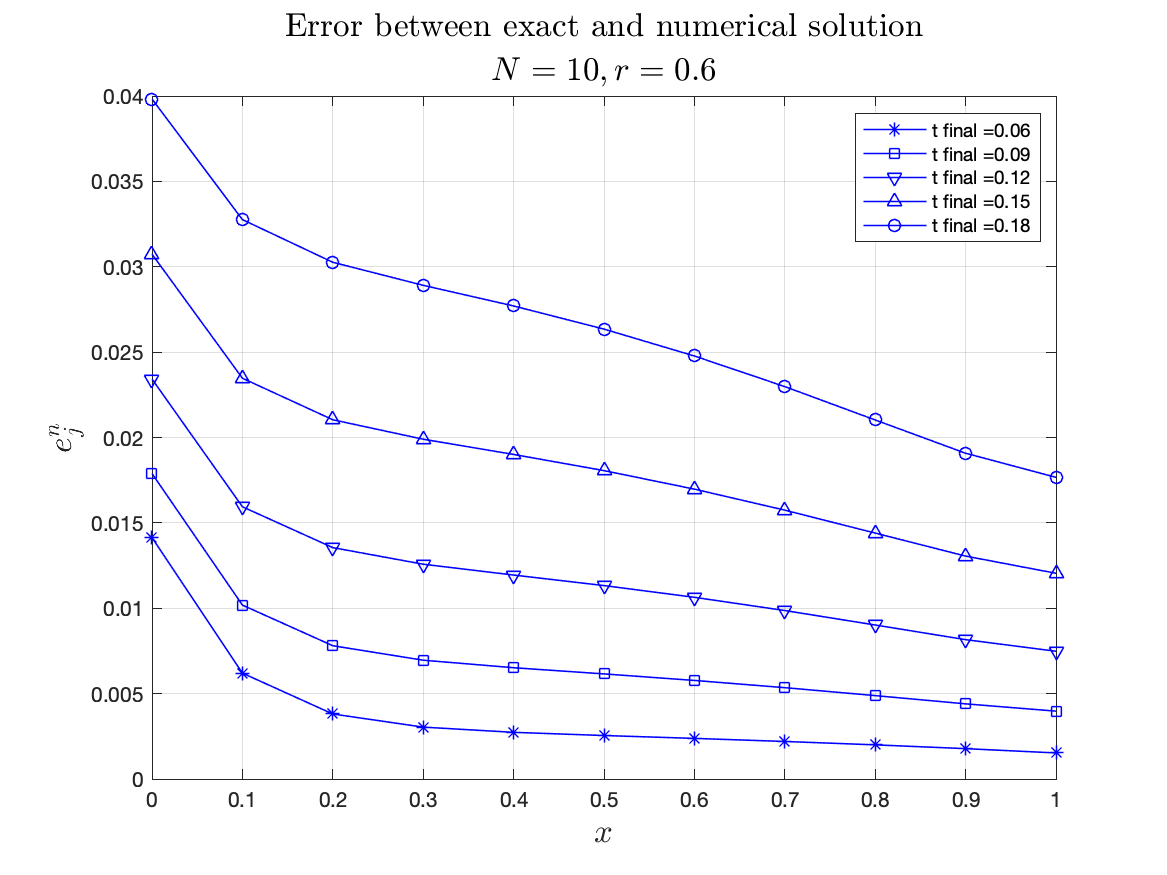
\includegraphics[width=4.5in]{Err_plot}
     \end{center}
     \label{fig:q1}
     \caption{Error between exact and numerical solution}
     \end{figure}
  %%%%%
  %%%%%
  %%%%%
  \item (10 pts.){ \color{red}Prove that the Lax-Friedrichs scheme}
    \begin{align*}
      v_j^{n+1} & =\frac{1}{2}(v_{j+1}^n+v_{j-1}^n)-\frac{R}{2}(v_{j+1}^n-v_{j-1}^n)
    \end{align*}
   { \color{red}is convergent in the max-norm to the solution of the PDE }$u_t+au_x=0${ \color{red} for }$|R|\le1$ {\color{red}with }$R=a\Delta t/\Delta x$. \\
   \begin{align*}
   \vnpj =  & \ \left(\frac{1-R}{2}\right)\vnjp + \left(\frac{1+R}{2}\right)\vnjm \\
   \text{Let, } \enj = & \ \vnj + \unj\\
   \text{(Assume } u & \text{ is smooth and } \unj \text{is a discrete value of } u \text{ in the spatial grid.)} \\
   \enpj & = \ \left(\frac{1-R}{2}\right)\enjp + \left(\frac{1+R}{2}\right)\enjm - \left\{ \unpj - \left(\frac{1-R}{2}\right)\unjp - \left(\frac{1+R}{2}\right)\unjm\right\}
   \end{align*}
   We can compute the truncation error as follows,
   \begin{align*}
   \unpj = & \ \texp{u + \dt \ut + \frac{\dt^2}{2!} u_{tt} + \frac{\dt^3}{3!} u_{ttt} + \Oc(\dt^4)}{n}{j} \\
   \unjp = & \ \texp{u + \dx \ux + \frac{\dx^2}{2!} \uxx + \frac{\dx^3}{3!} \uxxx + \Oc(\dx^4)}{n}{j} \\
   \unjm = & \ \texp{u - \dx \ux + \frac{\dx^2}{2!}\uxx - \frac{\dx^3}{3!}\uxxx + \Oc(\dx^4)}{j}{n} 
   \end{align*}
   
   \begin{align*}
   \unpj - \left(\frac{1-R}{2}\right)\unjp - & \left(\frac{1+R}{2}\right)\unjm =  \\
   & [{\color{blue}\dt \ut} + \frac{\dt^2}{2!}u_{tt} + \Oc(\dt^3) +  \\
   & {\color{blue}R\dx \ux} + R\frac{\dx^3}{3!}\uxxx + ... \ ... \\
   & - \frac{\dx^2}{2!}\uxx - \frac{\dx^4}{4!}\uxxxx + \Oc(\dx^6) ]^n_j
   \end{align*}
    Combining the terms in blue, we get, 
    \[
    \left(\dt \ u_t + R\dx \ \ux \right) = \dt \left(u_t + a\ux \right) = 0
    \]
    Now, combining this we get the truncation error to be, 
    \begin{align*}
    \unpj - \left(\frac{1-R}{2}\right)\unjp - \left(\frac{1+R}{2}\right)\unjm = & \ \Oc(\dt^2) + \Oc(\dt \dx^2) + \Oc(\dx^2) \approx A\left(\dt^2 + \dt \dx^2 + \dx^2\right) \\
    \tau^{n}_j & = A\left(\dt^2 + \dt \dx^2 + \dx^2\right)
    \end{align*}
    The error equation becomes,
    \begin{align*}
    \enpj & = \ \left(\frac{1-R}{2}\right)\enjp + \left(\frac{1+R}{2}\right)\enjm + \tau^{n}_{j} \\
     \enpj & = \ \left(\frac{1-R}{2}\right)\enjp + \left(\frac{1+R}{2}\right)\enjm + A\left(\dt^2 + \dt \dx^2 + \dx^2\right)
    \end{align*}
    Take the max norm of the above equation (absolute value) and set $E^n = \underset{j}{\text{max}} \ \enj$
    \begin{align*}
    \text{If, } k = 1 - R =& \ 1 + \left(-R\right) \text{ and, } 0 \leq (\modu{R} = m^2) \leq 1\\
    0\leq \modu{\frac{1-R}{2}} \leq & \ \frac{1}{2} \left(\modu{1} + \modu{-R} \right)\leq 1 \\
    \text{Similarly, } 0 \leq \modu{\frac{1+R}{2}} \leq & \ \frac{1}{2} \left(\modu{1}+\modu{R}\right) \leq 1\\
    \end{align*}
    \begin{align*}
    \modu{\enpj} \leq & \left(\frac{1-R}{2}\right)\modu{\enjp} + \left(\frac{1+R}{2}\right)\modu{\enjm} + A\left(\dt^2 + \dt \dx^2 + \dx^2\right) \\ \\
    E^{n+1} \leq & \ E^{n} + A\left(\dt^2 + \dt \dx^2 + \dx^2\right) \\
    \leq &\ E^{n-1} + 2A\left(\dt^2 + \dt \dx^2 + \dx^2\right) \\
    \leq & \ E^{n-2} + 3A\left(\dt^2 + \dt \dx^2 + \dx^2\right) \\
    & . \\
    & . \\
    \leq & \ E^0 + \left(n+1\right)A\left(\dt^2 + \dt \dx^2 + \dx^2\right) \\
    \leq & \ \left(n+1\right)A\left(\dt^2 + \dt \dx^2 + \dx^2\right), \ \text{as }E^0  = 0 \\
    \leq & \left(n+1\right)A\left(\frac{R^2}{a^2}\dx^2 + \frac{R}{a} \dx^3 + \dx^2\right) \rightarrow 0, \text{ as, }\dx \rightarrow 0
    \end{align*}
    Hence, it is convergent.
  %%%%%
  %%%%%
  %%%%%
  \item (10 pts.) {\color{red}Prove that the scheme}
    \[
      \Dpt v_j^n = \nu\Dpx\Dmx v_j^n+a\Dzx v_j^n
    \]
    {\color{red}is convergent in the max-norm to the solution of the PDE }$u_t= \nu u_{xx}+au_x${\color{red}, under certain constraints on }$\dx$ and $\dt${\color{red}. What are these constraints? Use the notation }$r=\nu\dt/\dx^2$ {\color{red}and} $\sigma=a\dt/\dx$.
    \begin{align*}
    \frac{\vnpj - \vnj}{\dt} = & \ \frac{\nu}{\dx^2}\left(\vnjp -2\vnj + \vnjm\right) + \frac{a}{2\dx}\left(\vnjp - \vnjm\right) \\
    \vnjp = & \ \vnj + r\left(\vnjp -2\vnj + \vnjm\right) + \frac{\sigma}{2}\left(\vnjp - \vnjm\right)\\
    \vnjp = & \ \left(r-\frac{\sigma}{2}\right)\vnjm + \left(1-2r\right)\vnj + \left(r+\frac{\sigma}{2}\right)\vnjp \\
    \vnjp = & \ \left(1-2r\right)\vnj + r\left[\vnjp + \vnjm\right] + \frac{\sigma}{2}\left(\vnjp - \vnjm\right) 
    \end{align*}
    Performing a DFT, 
    \begin{align*}
    \frac{1}{\sqrt{2\pi}}\sum_{j=-\infty}^{\infty} e^{-ij\xi}\vnpj = & \hat{V}^{n+1}\\
    \frac{1}{\sqrt{2\pi}}\sum_{j=-\infty}^{\infty} e^{-ij\xi}\vnj = & \  \hat{V}^{n} \\ 
    \frac{1}{\sqrt{2\pi}}\sum_{j=-\infty}^{\infty} e^{-i(j)\xi}\vnjp = & \ \frac{1}{\sqrt{2\pi}}\sum_{j=-\infty}^{\infty} e^{-i(m-1)\xi}v^n_m = e^{i\xi} \ \hat{V}^n \\
    \frac{1}{\sqrt{2\pi}}\sum_{j=-\infty}^{\infty} e^{-ij\xi}\vnjm =& \  e^{-i\xi}\hat{V}^n
    \end{align*}
    Substituting it into the equation,
    \begin{align*}
    \hat{V}^{n+1} = & \ \left(1-2r\right)\hat{V}^n + r\left[e^{i\xi} + e^{-i\xi}\right]\hat{V}^n + \frac{\sigma}{2}\left[e^{i\xi} - e^{-i\xi}\right]\hat{V}^n \\
    \hat{V}^{n+1} = & \ \left(1 - 2r + 2r\cos\xi + i\sigma\sin\xi\right)\hat{V}^n \\
    \hat{V}^{n+1} = & \ \left(1-2r\left(1-\cos\xi\right) + i\sigma\sin\xi\right)\hat{V}^n \\
    \modu{a(\xi)}^2 = & \left(1-2r\left(1-\cos\xi\right)\right)^2 + \left(\sigma\sin\xi\right)^2 \leq 1 \\
    \implies \modu{a(\xi)}^2 = &\ 1 + 4r^2\left(1-\cos\xi\right)^2 -4r\left(1-\cos\xi\right) + \sigma^2\left(1-\cos^2\xi\right) \leq 1 
    \end{align*}
    Let $z = \cos\xi$ 
\[
4r^2\left(1-z\right) -4r + \sigma^2\left(1+z\right) \leq 0
\]
If $z=-1$, $r\leq \frac{1}{2}$. \\
If $z = 1$, $\sigma^2 \leq 2r \leq 1$.\\
Therefore, the 2 constraints are,
\begin{align}
\dx^2 - a^2\dt^2 \geq 0 \\
\dx^2 -2\nu\dt \geq 0
\end{align}
  %%%%%
  %%%%%
  %%%%%
  \item (15 pts.) {\color{red}Determine the formal order of accuracy of the following difference equations (i.e. investigate the truncation error). Throughout, use the definitions }$r=\nu\dt/\dx^2$ {\color{red}and} $\sigma=a\dt/\dx$.
    \begin{enumerate}
      \item {\color{blue}For the PDE }$u_t= \nu u_{xx}-au_x$ {\color{blue}consider the discretization}
        \begin{align*}
         \Dpt v_j^n = \nu\Dpx\Dmx v_j^n-a\Dzx v_j^n.
        \end{align*}
        Let $\enj = \vnj - \unj$, 
        \begin{align*}
        \Dpt \left(\enj + \unj \right)= & \ \nu \Dpx\Dmx \left(\enj + \unj \right) -a\Dzx \left(\enj + \unj \right) \\
        \Dpt \enj = & \ \nu \Dpx\Dmx \enj -a\Dzx \enj -\left(\Dpt \unj - \nu \Dpx\Dmx \unj +a\Dzx \unj\right)
        \end{align*}
        \begin{align*}
        \Dpt \unj = & \  \texp{\ut + \frac{\dt}{2}u_{tt} + \Oc(\dt^2)}{n}{j} = \texp{\ut + \Oc(\dt)}{n}{j}\\
        \Dpx\Dmx \unj = & \ \texp{\uxx + \frac{\dx^2}{12}\uxxxx + \Oc(\dx^4)}{n}{j} = \texp{\uxx + \Oc(\dx^2)}{n}{j} \\
        \Dzx \unj = & \ \texp{\ux + \frac{\dx^2}{3!}\uxxx + \Oc(\dx^4)}{n}{j} = \texp{\ux + \Oc(\dx^2)}{n}{j}
        \end{align*}
        \begin{align*}
        \Dpt \enj = & \ \nu \Dpx\Dmx \enj -a\Dzx \enj - \left(\texp{{\color{blue}\ut - \nu \uxx + a\ux} + \Oc(\dt) + \Oc(\dx^2)}{n}{j}\right)
        \end{align*}
        The terms in blue sum up to 0 since it is the actual PDE. \\
        Therefore, truncation error is,
        \[
        \tau^n_j = \Oc(\dt) + \Oc(\dx^2)
        \]
        %%%
        %%%
      \item {\color{blue}For the PDE }$u_t= \nu u_{xx}-au_x$ {\color{blue}consider the discretization}
        \begin{align*}
          \Dpt v_j^n = \nu\Dpx\Dmx v_j^{n+1}-a\Dzx v_j^{n+1}.
        \end{align*}
        Similar to last problem,
        \begin{align*}
        \Dpt \enj = & \ \nu \Dpx\Dmx \enpj -a\Dzx \enpj -\left(\Dpt \unj - \nu \Dpx\Dmx \unpj +a\Dzx \unpj \right) \\
        \end{align*}
        \begin{align*}
        \Dpt \unj = & \  \texp{\ut + \frac{\dt}{2}u_{tt} + \Oc(\dt^2)}{n}{j} = \texp{\ut + \Oc(\dt)}{n}{j}\\
        \Dpx\Dmx \unpj = & \ \texp{\uxx + \frac{\dx^2}{12}\uxxxx + \Oc(\dx^4)}{n+1}{j} \\
        = & \ \texp{\uxx}{n+1}{j} + \frac{\dx^2}{12}\texp{\uxxxx}{n+1}{j} + \texp{\Oc(\dx^4)}{n+1}{j} \\
        = & \ \texp{\uxx + \dt \ u_{txx} + \Oc(\dt^2)}{n}{j} + \frac{\dx^2}{12}\texp{\uxxxx + \dt \ u_{txxxx} + \Oc(\dt^2)}{n}{j} + + \Oc(\dx^4)\\
        \Dzx \unpj = & \ \texp{\ux + \frac{\dx^2}{3!}\uxxx + \Oc(\dx^4)}{n+1}{j} \\
        = & \ \texp{\ux + \dt \ u_{tx} + \Oc(\dt^2)}{n}{j} + \frac{\dx^2}{3!} \texp{\uxxx + u_{txxx} + \Oc(\dt^2))}{n}{j} + \Oc(\dx^4) 
        \end{align*}
        \begin{align*}
        \Dpt\unj - \nu\Dpx\Dmx \unpj + a\Dzx\unpj = & \ \texp{{\color{blue}\ut - \nu\uxx + a\ux + \Oc(\dt) + \Oc(\dx^2)}}{n}{j}\\
        \tau^{n}_{j} = & \ \Oc(\dt) + \Oc(\dx^2)
        \end{align*}
        %%%
        %%%
      \item{ \color{blue}For the PDE }$u_t= -au_x${ \color{blue}consider the discretization}
        \begin{align*}
          \Dpt v_j^n = -a\Dmx v_j^{n+1}.
        \end{align*}
        Similar to the previous problem, 
        \begin{align*}
        \Dpt\enj = & -a\Dmx \enpj -\left( \Dpt\unj + a\Dmx\unpj \right)
        \end{align*}
        \begin{align*}
        \Dpt \unj = & \  \texp{\ut + \frac{\dt}{2}u_{tt} + \Oc(\dt^2)}{n}{j} = \texp{\ut + \Oc(\dt)}{n}{j}\\
        \Dmx\unpj = & \ \texp{\ux - \frac{\dx^2}{2!}\uxx + \frac{\dx^3}{3!}\uxxx + \Oc(\dx^4)}{n+1}{j}\\
        = & \ \texp{\ux + \dt u_{tx} + \Oc(\dt^2)}{n}{j} - \frac{\dx^2}{2!}\texp{\uxx + \dt u_{txx} + \Oc(\dt^2)}{n}{j}+ \Oc(\dx^4)\\
        \end{align*}
        \begin{align*}
        \tau^{n}_{j} = & \ \texp{{\color{blue}\ut + a\ux} + \Oc(\dt) + \Oc(\dx^2)}{n}{j} = \Oc(\dt) + \Oc(\dx^2)
        \end{align*}
    \end{enumerate}   
  %%%%%
  %%%%%
  %%%%%
  \item (15 pts.){\color{red} Investigate the stability of the schemes from number 4 above, and discuss any limitations on parameters that you find are required to guarantee stability. Again use the definitions }$r=\nu\dt/\dx^2$ {\color{red}and} $\sigma=a\dt/\dx${\color{red}. Hint: using the DFT is probably simplest.} \\
  
  I'm going to assume that the coefficients $\nu,a$ are positive in all three cases considered. So if, $\dt,\dx$ are set to be positive numbers, the parameters $r,\sigma$ are positive constants.
  
  \begin{enumerate}
  \item {\color{blue}For the PDE} $\ut = \nu\uxx - a\ux${\color{blue}, consider the discretization}
  \[
  \Dpt \vnj = \nu \Dpx\Dmx\vnj -a\Dzx\vnj
  \]
    \begin{align*}
    \frac{\vnpj - \vnj}{\dt} = & \ \frac{\nu}{\dx^2}\left(\vnjp -2\vnj + \vnjm\right) - \frac{a}{2\dx}\left(\vnjp - \vnjm\right) \\
    \vnjp = & \ \vnj + r\left(\vnjp -2\vnj + \vnjm\right) - \frac{\sigma}{2}\left(\vnjp - \vnjm\right)\\
    \vnjp = & \ \left(r+\frac{\sigma}{2}\right)\vnjm + \left(1-2r\right)\vnj + \left(r-\frac{\sigma}{2}\right)\vnjp \\
    \vnjp = & \ \left(1-2r\right)\vnj + r\left[\vnjp + \vnjm\right] - \frac{\sigma}{2}\left(\vnjp - \vnjm\right) 
    \end{align*}
    Performing a DFT, 
    \begin{align*}
    \frac{1}{\sqrt{2\pi}}\sum_{j=-\infty}^{\infty} e^{-ij\xi}\vnpj = & \hat{V}^{n+1}\\
    \frac{1}{\sqrt{2\pi}}\sum_{j=-\infty}^{\infty} e^{-ij\xi}\vnj = & \  \hat{V}^{n} \\ 
    \frac{1}{\sqrt{2\pi}}\sum_{j=-\infty}^{\infty} e^{-i(j)\xi}\vnjp = & \ \frac{1}{\sqrt{2\pi}}\sum_{j=-\infty}^{\infty} e^{-i(m-1)\xi}v^n_m = e^{i\xi} \ \hat{V}^n \\
    \frac{1}{\sqrt{2\pi}}\sum_{j=-\infty}^{\infty} e^{-ij\xi}\vnjm =& \  e^{-i\xi}\hat{V}^n
    \end{align*}
    Substituting it into the equation,
    \begin{align*}
    \hat{V}^{n+1} = & \ \left(1-2r\right)\hat{V}^n + r\left[e^{i\xi} + e^{-i\xi}\right]\hat{V}^n - \frac{\sigma}{2}\left[e^{i\xi} - e^{-i\xi}\right]\hat{V}^n \\
    \hat{V}^{n+1} = & \ \left(1 - 2r + 2r\cos\xi - i\sigma\sin\xi\right)\hat{V}^n \\
    \hat{V}^{n+1} = & \ \left(1-2r\left(1-\cos\xi\right) - i\sigma\sin\xi\right)\hat{V}^n \\
    \modu{a(\xi)}^2 = & \left(1-2r\left(1-\cos\xi\right)\right)^2 + \left(\sigma\sin\xi\right)^2 \leq 1 \\
    \implies \modu{a(\xi)}^2 = &\ 1 + 4r^2\left(1-\cos\xi\right)^2 -4r\left(1-\cos\xi\right) + \sigma^2\left(1-\cos^2\xi\right) \leq 1 
    \end{align*}
    Let $z = \cos\xi$ 
\[
4r^2\left(1-z\right) -4r + \sigma^2\left(1+z\right) \leq 0
\]
If $z=-1$, $r\leq \frac{1}{2}$. \\
If $z = 1$, $\sigma^2 \leq 2r \leq 1$.\\
If these conditions are met, then the scheme is stable. 
  %%%
  %%%
  \item {\color{blue}For the PDE} $\ut = \nu\uxx - a\ux${\color{blue}, consider the discretization}
  \[
  \Dpt \vnj = \nu \Dpx\Dmx\vnpj -a\Dzx\vnpj
  \]
    
  \begin{align*}
  \vnpj - \vnj = & \ \left(r - \frac{\sigma}{2}\right)\vnpjp - 2r\vnpj + \left(r+\frac{\sigma}{2}\right)\vnpjm
  \end{align*}
  Taking a DFT,
  \begin{align*}
  \frac{1}{\sqrt{2\pi}}\sum_{j=-\infty}^{\infty}e^{-ij\xi}\vnpjp =& \frac{1}{\sqrt{2\pi}}\sum_{m=-\infty}^{\infty}e^{-i(m-1)\xi}v^{n+1}_m \equiv e^{i\xi}\hat{V}^{n+1}\\
  \frac{1}{\sqrt{2\pi}}\sum_{j=-\infty}^{\infty}e^{-ij\xi}\vnpjm =& \frac{1}{\sqrt{2\pi}}\sum_{m=-\infty}^{\infty}e^{-i(m+1)\xi}v^{n+1}_m \equiv e^{-i\xi}\hat{V}^{n+1} \\
  \cos\xi = & \ \frac{e^{i\xi} + e^{-i\xi}}{2} \\
  \sin\xi = & \ \frac{e^{i\xi}-e^{-i\xi}}{2i}
  \end{align*}
  \begin{align*}
  \hVnp - \hVn = & \ \left(r-\frac{\sigma}{2}\right)e^{i\xi}\hVnp - 2r\hVnp + \left(r+ \frac{\sigma}{2}\right)e^{-i\xi}\hVnp \\
  \hVnp  = & \ \frac{1}{\left[1+2r(1-\cos\xi) + i\sigma\sin\xi\right]}\hVn \\ \\
  \implies a(\xi) = & \ \frac{\left[1+2r(1-\cos\xi) - i\sigma\sin\xi\right]}{(1+2r(1-\cos\xi))^2 + \sigma^2\sin^2\xi} \\ 
  \modu{a(\xi)}^2 = & \frac{1}{(1+2r(1-\cos\xi))^2 + \sigma^2\sin^2\xi} \\
  \end{align*}
  If $\modu{a(\xi)} \leq 1$, then this is a stable scheme.
  \begin{align*}
  \text{If, } & \cos\xi = -1, \\
  & 8r^2 + 4r \geq 0 \\
  & 4r(2r+1) \geq 0
  \end{align*}
  This is always true since we assumed $r\geq 0$
  \begin{align*}
  \text{If, } & \cos\xi = 1, \\
  & 4r + 2\sigma^2 \geq 0 
  \end{align*}
  This is also true since $r\geq 0$ and $\sigma \geq 0$.  Hence this is a stable scheme as $\modu{a(\xi)}\leq 1$ always.
  %%%
  %%%
  \item{ \color{blue}For the PDE }$u_t= -au_x${ \color{blue}consider the discretization}
        \begin{align*}
          \Dpt v_j^n = -a\Dmx v_j^{n+1}.
        \end{align*}
  \begin{align*}
  \vnpj - \vnj = & \ -\sigma \vnpj + \sigma \vnpjm \\
  \hVnp = & \ \frac{1}{1+\sigma\left(1-e^{-i\xi}\right)} \hVn \\
  e^{-i\xi} = & \cos\xi - i\sin\xi \\
  \implies \modu{a(\xi)}^2 = & \  \frac{1}{(1+\sigma(1-\cos\xi))^2+\sigma^2(1-\cos^2\xi)}
  \end{align*}
  The denominator is positive and always greater than 1, this stable is always stable since $\modu{a(\xi)}\leq 1$
  \end{enumerate}
  
\end{enumerate}

\end{document}
